% ============================================================
%  ROB-GY 6213  |  Final Project — Live 3-D Mapping with
%  Dynamic Obstacle Clearing
% ============================================================
\documentclass[aspectratio=169, 10pt]{beamer}
\usetheme{metropolis}
\usepackage{appendixnumberbeamer}

% ── packages ────────────────────────────────────────────────
\usepackage{tikz}
\usetikzlibrary{arrows.meta, positioning, calc,
                decorations.pathreplacing, backgrounds}
\usepackage{pgfplots}
\pgfplotsset{compat=1.18}
\usepackage{booktabs}
\usepackage{amsmath,amssymb}
\usepackage{graphicx}
\usepackage{xcolor}
\usepackage{multirow}
\usepackage{array}

% ── palette ─────────────────────────────────────────────────
\definecolor{nyu}{RGB}{87,6,140}
\definecolor{nvio}{RGB}{134,0,179}
\definecolor{sblue}{RGB}{0,114,189}
\definecolor{rust}{RGB}{200,70,30}
\definecolor{sage}{RGB}{34,130,80}
\definecolor{gold}{RGB}{190,145,0}
\definecolor{coal}{RGB}{40,40,40}
\definecolor{lgray}{RGB}{240,240,240}
\definecolor{mgray}{RGB}{180,180,180}

% ── metropolis overrides ─────────────────────────────────────
\setbeamercolor{normal text}{fg=coal, bg=white}
\setbeamercolor{frametitle}{bg=nyu, fg=white}
\setbeamercolor{title separator}{fg=nvio}
\setbeamercolor{progress bar}{fg=nvio, bg=mgray!60}
\setbeamercolor{alerted text}{fg=rust}
\setbeamercolor{example text}{fg=sblue}
\setbeamercolor{block title}{bg=nyu!12, fg=nyu!80!black}
\setbeamercolor{block body}{bg=nyu!5}
\setbeamercolor{block title alerted}{bg=rust!15, fg=rust!75!black}
\setbeamercolor{block body alerted}{bg=rust!5}
\setbeamercolor{block title example}{bg=sblue!13, fg=sblue!80!black}
\setbeamercolor{block body example}{bg=sblue!5}
\metroset{block=fill, progressbar=frametitle,
          sectionpage=none, numbering=fraction}
\setbeamerfont{frametitle}{size=\normalsize, series=\bfseries}
\setbeamerfont{block title}{size=\small, series=\bfseries}
\setlength{\leftmargini}{1.1em}
\setlength{\leftmarginii}{1.0em}

% ── macros ───────────────────────────────────────────────────
\newcommand{\xh}{\hat{\mathbf{x}}}
\newcommand{\Pk}{\mathbf{P}}
\newcommand{\Rk}{\mathbf{R}}
\newcommand{\Qk}{\mathbf{Q}}
% purple numbered circle
\newcommand{\cn}[1]{%
  \tikz[baseline=(x.base),inner sep=0pt]
    \node[circle,fill=nyu,text=white,font=\scriptsize\bfseries,
          minimum size=15pt](x){#1};\,%
}

% ── title info ────────────────────────────────────────────────
\title{Live 3-D Mapping with Dynamic Obstacle Clearing\\
       for Autonomous Navigation in Unknown Environments}
\subtitle{ROB-GY 6213 \;·\; Final Project}
\author{[Your Names Here]}
\institute{New York University \;·\; Tandon School of Engineering}
\date{May 5, 2026}

% ============================================================
\begin{document}
% ============================================================

\maketitle

% ── SLIDE 1: INTRODUCTION ───────────────────────────────────
\begin{frame}{Introduction}
\begin{columns}[T]

  \column{0.52\textwidth}
  \textbf{Scenario}\\[3pt]
  \small
  A wheeled service robot enters a \alert{completely unseen} indoor
  environment and must reach goals with \emph{no prior map},
  while people and objects intermittently block the path.

  \vspace{5pt}
  \normalsize\textbf{Key challenges}
  \begin{itemize}\small
    \item Build a globally-consistent 3-D map from scratch
    \item Detect and avoid dynamic obstacles in real time
    \item \alert{Clear} transient objects from the map once they
          leave — so future paths stay optimal
  \end{itemize}

  \vspace{5pt}
  \begin{exampleblock}{\small Why clearing matters long-term}
    \small Without clearing, repeated deployments accumulate
    ``ghost'' obstacles that permanently degrade paths.
    Active clearing keeps the map trustworthy for semantic
    SLAM, loop closure, and multi-session planning.
  \end{exampleblock}

  \column{0.45\textwidth}
  \vspace{4pt}
  \centering
  % ── scenario sketch ──
  % natural size: 5.5 wide × 3.6 tall  (aspect 1.53)
  % in 0.45 col with resizebox{0.96\linewidth}: ~5.1 × 3.3 cm  ✓
  \resizebox{0.96\linewidth}{!}{%
  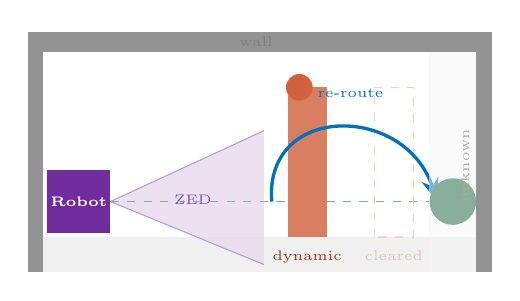
\begin{tikzpicture}[>=Stealth, thick, font=\small]
    % floor / ceiling
    \fill[lgray]        (-0.2,-0.45) rectangle (5.7, 0.0);
    \fill[coal!50]      (-0.2, 2.35) rectangle (5.7, 2.60);
    \fill[coal!50]      (-0.2,-0.45) rectangle (0.0, 2.60);
    \fill[coal!50]      (5.50,-0.45) rectangle (5.70, 2.60);
    \node[font=\tiny,coal!60] at (2.7,2.48) {wall};

    % robot body
    \fill[nyu!85]   (0.05, 0.05) rectangle (0.85, 0.85);
    \node[font=\tiny\bfseries,white] at (0.45,0.45) {Robot};

    % sensor frustum
    \fill[nyu!15,opacity=0.8]
      (0.85,0.45) -- (2.8,1.35) -- (2.8,-0.35) -- cycle;
    \draw[nyu!40,thin] (0.85,0.45)--(2.8,1.35);
    \draw[nyu!40,thin] (0.85,0.45)--(2.8,-0.35);
    \node[font=\tiny,nyu!70] at (1.9,0.47) {ZED};

    % original path (dashed sage)
    \draw[sage!60, dashed, thin]
      (0.85,0.45) -- (3.0,0.45) -- (4.9,0.45);

    % dynamic obstacle
    \fill[rust!70]  (3.1, 0.0) rectangle (3.6, 1.90);
    \fill[rust!85]  (3.25,1.90) circle (0.17);
    \node[font=\tiny,rust!80!black,below] at (3.35,-0.05) {dynamic};

    % ghost / cleared
    \draw[rust!25, dashed, thin]
      (4.2, 0.0) rectangle (4.7, 1.90);
    \node[font=\tiny,rust!35,below] at (4.45,-0.05) {cleared};

    % re-routed path
    \draw[sblue, very thick, -Stealth]
      (2.9,0.45) .. controls (2.8,1.7) and (4.6,1.7) .. (5.0,0.45);
    \node[font=\tiny,sblue] at (3.9,1.82) {re-route};

    % goal
    \node[draw=sage,fill=sage!20,circle,minimum size=13pt,
          font=\tiny\bfseries,sage!80!black] at (5.2,0.45) {G};

    % unknown region
    \fill[lgray!60,opacity=0.5] (4.9,-0.45) rectangle (5.50,2.35);
    \node[font=\tiny,coal!40,rotate=90] at (5.35,0.9) {unknown};
  \end{tikzpicture}
  }%
\end{columns}
\end{frame}

% ── SLIDE 2: PROBLEM DEFINITION ─────────────────────────────
\begin{frame}{Problem Definition}
\begin{columns}[T]

  \column{0.43\textwidth}
  \textbf{State vector} $\mathbf{x}_k$
  \[
    \mathbf{x}_k =
    \begin{bmatrix}p_x \\ p_z \\ \psi\end{bmatrix}_{\!k}
    \;\in\;\mathbb{R}^2\!\times[-\pi,\pi)
  \]
  \footnotesize 2-D position + heading, world XZ-plane (Y-up)

  \vspace{6pt}
  \normalsize\textbf{Input measurements}
  \begin{itemize}\small
    \item \textbf{Encoders} $\mathbf{u}_k$:
          $\Delta p_x,\,\Delta p_z,\,\Delta\psi$ at 20\,Hz
    \item \textbf{ZED VIO} $\mathbf{z}_k$:
          6-DOF pose $(x,y,z,\mathbf{q})$ at 30\,Hz\\
          \quad + confidence score $\in[0,100]$
    \item \textbf{Point cloud} $\mathcal{P}_k$:
          40k–200k pts at 30\,Hz
  \end{itemize}

  \vspace{6pt}
  \textbf{Intermediate variables}
  \begin{itemize}\small
    \item TSDF voxel map $\mathcal{V}$ (3\,cm voxels)
    \item 2-D occupancy grid $\mathcal{G}_k$ (5\,cm cells)
    \item Per-voxel TTL counter $\tau\;\in\{0,\ldots,25\}$
  \end{itemize}

  \column{0.55\textwidth}
  \vspace{-4pt}
  \centering
  % ── coordinate frame diagram ──
  % natural: 9.0 wide × 5.6 tall  (aspect 1.61)
  % in 0.55 col with \resizebox{0.97\linewidth}: ~6.8 × 4.2 cm  ✓
  \resizebox{0.97\linewidth}{!}{%
  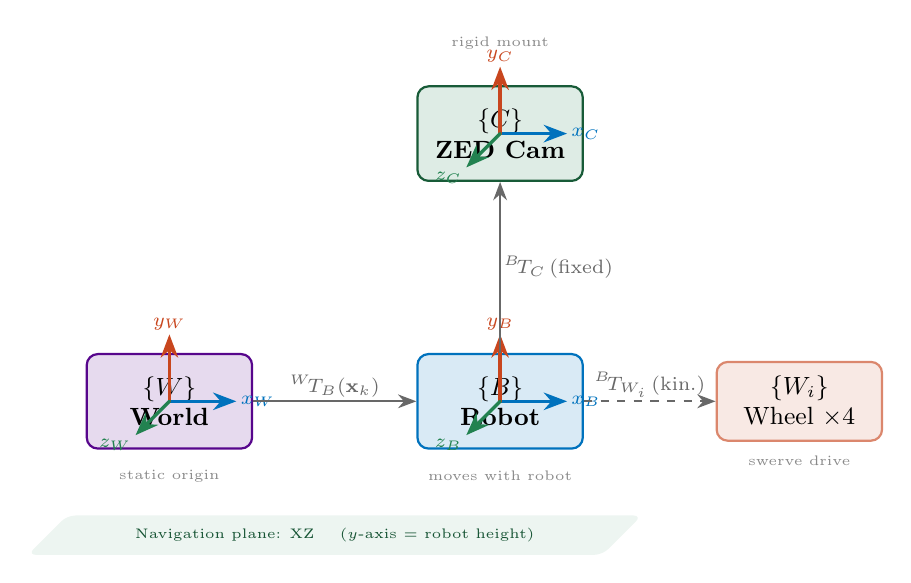
\begin{tikzpicture}[
    frm/.style={draw,thick,rounded corners=4pt,
                minimum width=2.1cm, minimum height=1.2cm,
                align=center, font=\small\bfseries},
    ax/.style={-Stealth,very thick,line cap=round},
    tf/.style={-Stealth,thick,coal!70},
    lb/.style={font=\scriptsize,inner sep=1pt},
    >=Stealth
  ]
    %% World ──────────────────────────────────
    \node[frm, fill=nyu!15, draw=nyu]   (W) at (0,0) {$\{W\}$\\World};
    \draw[ax,sblue]  (W.center) -- ++(0.85,0)  node[right,lb,sblue]{$x_W$};
    \draw[ax,rust]   (W.center) -- ++(0,0.85)  node[above,lb,rust]{$y_W$};
    \draw[ax,sage]   (W.center) -- ++(-.43,-.43) node[below left,lb,sage]{$z_W$};
    \node[font=\tiny,coal!55] at (0,-0.95) {static origin};

    %% Robot Base ─────────────────────────────
    \node[frm, fill=sblue!15, draw=sblue] (B) at (4.2,0) {$\{B\}$\\Robot};
    \draw[ax,sblue]  (B.center) -- ++(0.85,0)  node[right,lb,sblue]{$x_B$};
    \draw[ax,rust]   (B.center) -- ++(0,0.85)  node[above,lb,rust]{$y_B$};
    \draw[ax,sage]   (B.center) -- ++(-.43,-.43) node[below left,lb,sage]{$z_B$};
    \node[font=\tiny,coal!55] at (4.2,-0.95) {moves with robot};

    \draw[tf] (W.east) -- (B.west)
          node[midway,above,lb]{${}^W\!T_B(\mathbf{x}_k)$};

    %% Camera ─────────────────────────────────
    \node[frm, fill=sage!15, draw=sage!70!black] (C) at (4.2,3.4)
          {$\{C\}$\\ZED Cam};
    \draw[ax,sblue]  (C.center) -- ++(0.85,0)  node[right,lb,sblue]{$x_C$};
    \draw[ax,rust]   (C.center) -- ++(0,0.85)  node[above,lb,rust]{$y_C$};
    \draw[ax,sage]   (C.center) -- ++(-.43,-.43) node[below left,lb,sage]{$z_C$};
    \node[font=\tiny,coal!55] at (4.2,4.55) {rigid mount};

    \draw[tf] (B.north) -- (C.south)
          node[midway,right,lb]{${}^B\!T_C$\,(fixed)};

    %% Wheels ──────────────────────────────────
    \node[frm, fill=rust!12, draw=rust!65,
          minimum width=2.1cm, minimum height=1.0cm,
          font=\small] (Wi) at (8.0,0) {$\{W_i\}$\\Wheel $\times4$};
    \draw[tf,dashed] (B.east) -- (Wi.west)
          node[midway,above,lb]{${}^B\!T_{W_i}$\,(kin.)};
    \node[font=\tiny,coal!55] at (8.0,-0.75) {swerve drive};

    %% Navigation plane annotation ─────────────
    \begin{scope}[on background layer]
      \fill[sage!8, rounded corners=3pt]
        (-1.3,-1.45) -- (6.0,-1.45) --
        (5.5,-1.95)  -- (-1.8,-1.95) -- cycle;
    \end{scope}
    \node[font=\tiny,sage!65!black] at (2.1,-1.70)
          {Navigation plane: XZ \quad ($y$-axis = robot height)};

  \end{tikzpicture}
  }%
\end{columns}
\end{frame}

% ── SLIDE 3: DATA & SENSORS ─────────────────────────────────
\begin{frame}{Data \& Sensor Suite}
\begin{columns}[T]

  \column{0.48\textwidth}
  \begin{block}{ZED\,2 Stereo-Depth Camera}
    \small\renewcommand{\arraystretch}{1.1}
    \begin{tabular}{@{}ll@{}}
      Rate          & 30\,Hz \\
      Resolution    & VGA 640$\times$480 \\
      Depth mode    & \texttt{NEURAL} (AI-stereo) \\
      Range         & 0.5 – 8\,m \\
      Pose output   & 6-DOF VIO + confidence\\
      Conf.\ thresh & 87\% depth \;|\; 95\% texture \\
    \end{tabular}
  \end{block}

  \vspace{5pt}
  \begin{block}{Swerve Drive Encoders}
    \small\renewcommand{\arraystretch}{1.1}
    \begin{tabular}{@{}ll@{}}
      Wheels      & 4 independent steer + drive \\
      Rate        & 20\,Hz \\
      Calibration & 0.04992\,m\,/\,revolution \\
      Geometry    & WB\,145\,mm, track\,202\,mm \\
      Kinematics  & Least-squares FK (4-eq.\ → 3-DOF) \\
    \end{tabular}
  \end{block}

  \column{0.50\textwidth}
  \begin{exampleblock}{Point Cloud Pipeline}
    \small\renewcommand{\arraystretch}{1.1}
    \begin{tabular}{@{}ll@{}}
      Raw density  & 40k – 200k pts\,/\,frame \\
      Height band  & $[0.30,\;1.50]$\,m (obstacle) \\
      Voxel size   & 3\,cm (map) \\
      Grid cell    & 5\,cm (2-D planner) \\
    \end{tabular}
  \end{exampleblock}

  \vspace{5pt}
  \begin{alertblock}{Characterised Operational Limits}
    \small\renewcommand{\arraystretch}{1.1}
    \begin{tabular}{@{}ll@{}}
      Min.\ obstacle height & \textbf{30\,cm} \\
      Min.\ avoidance dist. & \textbf{$\approx$35\,cm} \\
      Path inflation radius & 30\,cm \\
    \end{tabular}
    \vspace{2pt}\\
    \footnotesize Both limits verified through dedicated
    experiments separate from the main benchmark.
  \end{alertblock}

\end{columns}
\end{frame}

% ── SLIDE 4: EKF STATE ESTIMATOR ────────────────────────────
\begin{frame}{State Estimator: Adaptive Sensor-Fused EKF}
\begin{columns}[T]

  \column{0.50\textwidth}
  \small\textbf{Filter class:} EKF \cite{kalman1960new,thrun2005probabilistic}

  \vspace{3pt}
  \textbf{Predict} (encoder dead-reckoning, 20\,Hz):
  \begin{align*}
    \xh_{k|k-1} &= f(\mathbf{x}_{k-1},\mathbf{u}_k) \\
    \Pk_{k|k-1} &= \mathbf{F}\Pk_{k-1}\mathbf{F}^\top + \Qk_k
  \end{align*}

  \vspace{-2pt}
  \textbf{Update} (ZED VIO, 30\,Hz):
  \begin{align*}
    \mathbf{K}_k &= \Pk_{k|k-1}\mathbf{H}^\top
                   \!\bigl(\mathbf{H}\Pk_{k|k-1}\mathbf{H}^\top
                   +\Rk_k\bigr)^{-1}\\
    \Pk_k &= (\mathbf{I}-\mathbf{K}_k\mathbf{H})\Pk_{k|k-1}
             (\mathbf{I}-\mathbf{K}_k\mathbf{H})^\top
             +\mathbf{K}_k\Rk_k\mathbf{K}_k^\top
  \end{align*}
  \vspace{-4pt}
  \footnotesize Joseph form — numerically stable covariance update.

  \vspace{4pt}
  \normalsize\textbf{Adaptive measurement noise:}
  \[
    \Rk_k = \Rk_0\cdot\!\left(\tfrac{100}{\text{conf}_k+1}\right)^{\!\alpha}
  \]
  \footnotesize Automatically down-weights VIO in poor conditions\\
  (low light, fast motion, textureless surfaces).

  \column{0.48\textwidth}
  \vspace{2pt}
  \begin{block}{vs.\ Standard EKF \cite{thrun2005probabilistic}}
    \small\renewcommand{\arraystretch}{1.15}
    \begin{tabular}{@{}lcc@{}}
      \toprule
      Feature & Std. & \textbf{Ours} \\
      \midrule
      Measurement noise $\Rk$ & fixed & \alert{adaptive} \\
      Zero-vel.\ update (ZUPT) & $\times$ & \checkmark \\
      Mahalanobis gating & opt. & \checkmark \\
      Joseph-form $\Pk$ & $\times$ & \checkmark \\
      Surface-tuned $\Qk$ & $\times$ & \checkmark \\
      \bottomrule
    \end{tabular}
  \end{block}

  \vspace{6pt}
  \begin{alertblock}{Carpet-specific process noise}
    \small $\Qk$ tuned $3\text{–}4\times$ harder-floor values to account
    for swerve wheel compression and lateral slip on carpet.
  \end{alertblock}

  \vspace{6pt}
  \begin{exampleblock}{ZUPT condition}
    \small When encoder speed $\approx 0$, a zero-velocity pseudo-measurement
    is injected to prevent covariance growth during standstill.
  \end{exampleblock}

\end{columns}
\end{frame}

% ── SLIDE 5: SYSTEM BLOCK DIAGRAM ───────────────────────────
\begin{frame}{System Architecture}
\vspace{-2pt}
\centering
% natural: 12.0 wide × 4.6 tall  (aspect 2.61)
% \resizebox{\textwidth}{!}: ~12.8 × 4.9 cm  ✓
\resizebox{\textwidth}{!}{%
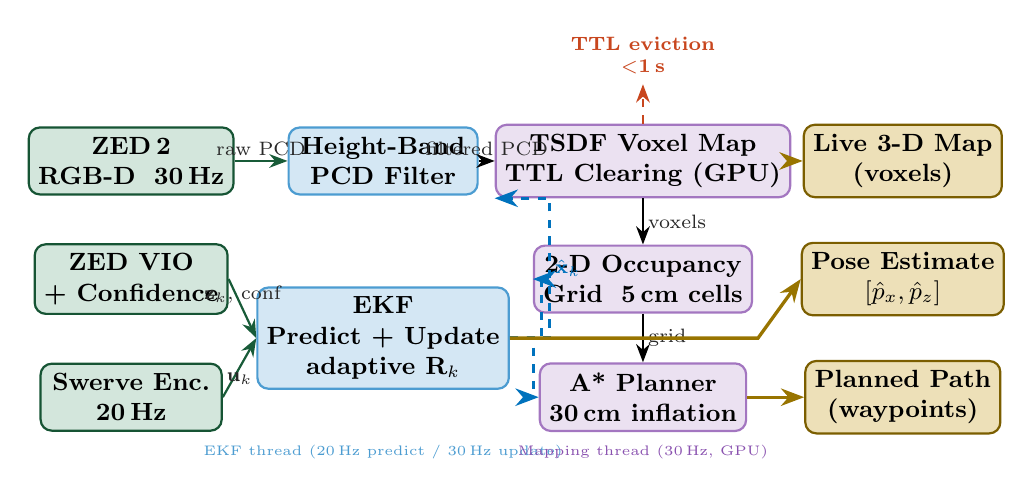
\begin{tikzpicture}[
  S/.style={draw,thick,rounded corners=4pt,
            minimum width=2.3cm,minimum height=0.85cm,
            align=center,font=\small\bfseries,
            fill=sage!20,draw=sage!65!black},
  P/.style={draw,thick,rounded corners=4pt,
            minimum width=2.4cm,minimum height=0.85cm,
            align=center,font=\small\bfseries,
            fill=sblue!17,draw=sblue!70},
  M/.style={draw,thick,rounded corners=4pt,
            minimum width=2.4cm,minimum height=0.85cm,
            align=center,font=\small\bfseries,
            fill=nyu!12,draw=nyu!55},
  O/.style={draw,thick,rounded corners=4pt,
            minimum width=2.3cm,minimum height=0.85cm,
            align=center,font=\small\bfseries,
            fill=gold!28,draw=gold!65!black},
  ar/.style={-Stealth,thick},
  lb/.style={font=\scriptsize,coal,inner sep=1.5pt},
  >=Stealth
]

%% col-x:  0 | 3.2 | 6.5 | 9.8
%% row-y:  3.2 | 1.7 | 0.2

% sensors
\node[S] (RGB) at (0,  3.2) {ZED\,2\\RGB-D \;30\,Hz};
\node[S] (VIO) at (0,  1.7) {ZED VIO\\+ Confidence};
\node[S] (ENC) at (0,  0.2) {Swerve Enc.\\20\,Hz};

% processing col 1
\node[P] (HF)  at (3.2, 3.2) {Height-Band\\PCD Filter};
\node[P] (EKF) at (3.2, 0.95) {\textbf{EKF}\\Predict + Update\\adaptive $\Rk_k$};

% processing col 2
\node[M] (TSDF) at (6.5, 3.2) {TSDF Voxel Map\\TTL Clearing (GPU)};
\node[M] (GRID) at (6.5, 1.7) {2-D Occupancy\\Grid \;5\,cm cells};
\node[M] (PLAN) at (6.5, 0.2) {A* Planner\\30\,cm inflation};

% outputs
\node[O] (OM)  at (9.8, 3.2) {Live 3-D Map\\(voxels)};
\node[O] (OP)  at (9.8, 1.7) {Pose Estimate\\$[\hat{p}_x,\hat{p}_z]$};
\node[O] (OW)  at (9.8, 0.2) {Planned Path\\(waypoints)};

% sensor → proc col1
\draw[ar,sage!70!black] (RGB.east) -- (HF.west)
      node[midway,above,lb]{raw PCD};
\draw[ar,sage!70!black] (VIO.east) -- (EKF.west)
      node[midway,above,lb]{$\mathbf{z}_k$, conf};
\draw[ar,sage!70!black] (ENC.east) -- (EKF.west)
      node[midway,below,lb]{$\mathbf{u}_k$};

% proc col1 → col2
\draw[ar] (HF.east) -- (TSDF.west)
      node[midway,above,lb]{filtered PCD};
\draw[ar] (TSDF.south) -- (GRID.north)
      node[midway,right,lb]{voxels};
\draw[ar] (GRID.south) -- (PLAN.north)
      node[midway,right,lb]{grid};

% EKF pose → col2 (dashed)
\draw[ar,sblue,dashed,very thick]
      (EKF.east) -- ++(0.5,0) |- (TSDF.south west)
      node[near start,right,lb,sblue]{$\xh_k$};
\draw[ar,sblue,dashed,very thick]
      (EKF.east) -- ++(0.4,0) |- (GRID.west);
\draw[ar,sblue,dashed,very thick]
      (EKF.east) -- ++(0.3,0) |- (PLAN.west);

% col2 → outputs
\draw[ar,gold!80!black,very thick] (TSDF.east) -- (OM.west);
\draw[ar,gold!80!black,very thick]
      (EKF.east) -- ++(3.15,0) -- (OP.west);
\draw[ar,gold!80!black,very thick] (PLAN.east) -- (OW.west);

% TTL annotation
\draw[-Stealth,rust,thick,dashed]
      (TSDF.north) -- ++(0,0.5)
      node[above,font=\scriptsize\bfseries,rust,align=center]
      {TTL eviction\\$<$1\,s};

% thread labels
\node[font=\tiny,sblue!70] at (3.2,-0.5)
      {EKF thread (20\,Hz predict / 30\,Hz update)};
\node[font=\tiny,nyu!70]   at (6.5,-0.5)
      {Mapping thread (30\,Hz, GPU)};

\end{tikzpicture}
}%
\end{frame}

% ── SLIDE 6: DYNAMIC CLEARING ───────────────────────────────
\begin{frame}{Live Mapping \& Dynamic Obstacle Clearing}
\begin{columns}[T]

  \column{0.50\textwidth}
  \textbf{TSDF voxel map} \cite{newcombe2011kinectfusion}
  \begin{itemize}\small
    \item KinectFusion-style: free-space carving + log-odds updates
    \item 3\,cm voxels; GPU-accelerated (PyTorch/CUDA)
    \item Color EMA per voxel for textured reconstruction
  \end{itemize}

  \vspace{5pt}
  \textbf{TTL clearing algorithm}
  \begin{enumerate}\small
    \item Transform $\mathcal{P}_k$ to world frame via $\xh_k$
    \item \textbf{Free-space ray-march}: decrement log-odds
          and $\tau$ along each ray
    \item \textbf{Hit voxel}: increment log-odds;
          reset $\tau\!\leftarrow\!25$
    \item \textbf{Evict}: remove voxels with $\tau=0$
  \end{enumerate}

  \vspace{5pt}
  \small
  \alert{Walls/floors} — re-observed every frame
  $\Rightarrow$ $\tau$ stays at 25 $\Rightarrow$ \textbf{persist}\\[3pt]
  \alert{Moving people} — leave FoV
  $\Rightarrow$ $\tau$ expires in $<$1\,s $\Rightarrow$ \textbf{cleared}

  \column{0.48\textwidth}
  \begin{block}{vs.\ Standard Occupancy Maps}
    \small\renewcommand{\arraystretch}{1.1}
    \begin{tabular}{@{}p{3.2cm}cc@{}}
      \toprule
      Property & Std. & \textbf{Ours} \\
      \midrule
      Dynamic clearing       & $\times$ & \checkmark \\
      Absence = evidence     & $\times$ & \checkmark \\
      Single map layer       & \checkmark & \checkmark \\
      Real-time (GPU)        & opt. & \checkmark \\
      \bottomrule
    \end{tabular}
  \end{block}

  \vspace{5pt}
  \begin{exampleblock}{Path Re-planning}
    \small A* re-runs on the live grid each cycle. Once an obstacle
    clears, the optimal path is restored automatically — no human
    intervention required.
  \end{exampleblock}

  \vspace{5pt}
  \begin{alertblock}{Long-term benefit}
    \small Transient objects never permanently pollute the map,
    enabling semantic SLAM and loop-closure over extended
    deployments from a single consistent map.
  \end{alertblock}

\end{columns}
\end{frame}

% ── SLIDE 7: EXPERIMENTS ────────────────────────────────────
\begin{frame}{Experiments}
\begin{columns}[T]

  \column{0.50\textwidth}
  \textbf{Benchmark protocol}
  \begin{itemize}\small
    \item \textbf{5 round-trip runs} (A$\leftrightarrow$B),
          indoor corridor; A–B straight-line: \textbf{4.98\,m}
    \item 4 conditions (full factorial):
  \end{itemize}
  \vspace{3pt}
  \small\renewcommand{\arraystretch}{1.1}
  \begin{tabular}{@{}clcc@{}}
    \toprule
    & Condition & EKF & Obstacles \\
    \midrule
    1 & EKF + obstacles     & \checkmark & \checkmark \\
    2 & EKF, no obstacles   & \checkmark & $\times$ \\
    3 & ZED-only + obstacles & $\times$  & \checkmark \\
    4 & ZED baseline        & $\times$   & $\times$ \\
    \bottomrule
  \end{tabular}

  \vspace{8pt}
  \normalsize\textbf{Characterisation tests}
  \begin{itemize}\small
    \item Height sweep: \textbf{30\,cm} min.\ detectable obstacle
    \item Avoidance margin: \textbf{$\approx$35\,cm} min.\ safe distance
  \end{itemize}

  \column{0.48\textwidth}
  \textbf{Performance metric — RMS position error}
  \[
    e_{\mathrm{RMS}} =
    \sqrt{\frac{1}{N}\sum_{k=1}^{N}
      \bigl\|\hat{\mathbf{p}}_k^{\mathrm{arr}}
             -\mathbf{p}_k^{\mathrm{ref}}\bigr\|^2}
  \]
  \footnotesize $N=10$ legs; $\mathbf{p}^{\mathrm{ref}}$ = mean arrival
  position across ZED-baseline runs (condition 4).

  \vspace{6pt}
  \normalsize
  \begin{block}{Results summary}
    \small\renewcommand{\arraystretch}{1.15}
    \begin{tabular}{@{}lcc@{}}
      \toprule
      Condition & $e_{\mathrm{RMS}}$ & Speed \\
      \midrule
      \textbf{EKF + obs}  & \textbf{3.29\,cm} & \textbf{0.238\,m/s} \\
      EKF, no obs         & 2.74\,cm & 0.208\,m/s \\
      ZED + obs           & 3.52\,cm & 0.157\,m/s \\
      ZED baseline        & 2.32\,cm & 0.160\,m/s \\
      \bottomrule
    \end{tabular}
  \end{block}
  \vspace{3pt}
  \footnotesize EKF: \alert{52\% faster} than ZED-only with obstacles;
  $e_{\mathrm{RMS}}$ stays $<3.3$\,cm.

\end{columns}
\end{frame}

% ── SLIDE 8: RESULTS — single plot ──────────────────────────
\begin{frame}{Results: EKF with Dynamic Obstacles}
  \begin{center}
    \includegraphics[width=0.80\textwidth, keepaspectratio]%
                    {benchmark_ekf_w_objects_plots.png}
  \end{center}
  \vspace{-4pt}
  \footnotesize
  EKF condition, 5 runs, 10 legs.
  \textbf{Trajectory:} tight clustering; max positional deviation $<4.51$\,cm.
  \textbf{Per-leg error:} all arrival errors $<5$\,cm.
  \textbf{Uncertainty:} $\sigma_x\!\approx\!10\text{–}20$\,mm,
  $\sigma_z\!\approx\!15\text{–}30$\,mm throughout mission.
\end{frame}

% ── SLIDE 9: RESULTS — comparison ───────────────────────────
\begin{frame}{Results: EKF vs.\ ZED-Only Under Dynamic Obstacles}
  \begin{columns}[T]
    \column{0.496\textwidth}
    \centering
    \small\textbf{EKF fusion + dynamic obstacles}\\[4pt]
    \includegraphics[width=\textwidth, keepaspectratio]%
                    {benchmark_ekf_w_objects_plots.png}\\[3pt]
    \footnotesize
    $e_{\mathrm{RMS}}=3.29$\,cm\quad Speed\,$=0.238$\,m/s

    \column{0.496\textwidth}
    \centering
    \small\textbf{ZED-only + dynamic obstacles}\\[4pt]
    \includegraphics[width=\textwidth, keepaspectratio]%
                    {benchmark_no_ekf_w_objects_plots.png}\\[3pt]
    \footnotesize
    $e_{\mathrm{RMS}}=3.52$\,cm\quad Speed\,$=0.157$\,m/s
  \end{columns}
  \vspace{5pt}
  \small
  EKF fusion: \alert{$-7\%$ position error} and \alert{$+52\%$ speed}
  under identical conditions.
  Smoother pose estimates reduce unnecessary replanning pauses.
\end{frame}

% ── SLIDE 10: CONCLUSIONS ───────────────────────────────────
\begin{frame}{Conclusions}
  \setlength\itemsep{5pt}
  \begin{enumerate}

    \item[\cn{1}] \textbf{Real-time dynamic clearing is feasible on a
          mobile platform.}\\
          \small GPU TSDF + 25-frame TTL evicts transient obstacles
          in $<$1\,s at camera rate — enabling zero-prior-map navigation
          without manual map resets.

    \item[\cn{2}] \textbf{EKF fusion improves speed without sacrificing
          accuracy.}\\
          \small Adaptive-$\Rk$ EKF achieved 52\% higher navigational speed
          over ZED-only (0.238 vs.\ 0.157\,m/s) while keeping
          $e_{\mathrm{RMS}}<3.3$\,cm with dynamic obstacles present.

    \item[\cn{3}] \textbf{Active clearing is essential for long-term map
          fidelity.}\\
          \small Without TTL clearing, transient objects permanently degrade
          paths across sessions; our system self-corrects, supporting
          semantic SLAM and loop closure.

    \item[\cn{4}] \textbf{Operational limits are characterised and
          predictable.}\\
          \small Min.\ detectable height 30\,cm; safe avoidance margin
          $\approx$35\,cm — clear bounds that directly inform deployment
          decisions.

  \end{enumerate}
\end{frame}

% ── SLIDE 11: REFERENCES ────────────────────────────────────
\begin{frame}[allowframebreaks]{References}
  \footnotesize
  \begin{thebibliography}{9}

    \bibitem{kalman1960new}
    R.~E. Kalman, ``A new approach to linear filtering and prediction
    problems,'' \emph{J.\ Basic Eng.}, vol.~82, no.~1,
    pp.~35--45, 1960.

    \bibitem{thrun2005probabilistic}
    S.~Thrun, W.~Burgard, and D.~Fox,
    \emph{Probabilistic Robotics}. MIT Press, 2005.

    \bibitem{newcombe2011kinectfusion}
    R.~A. Newcombe \emph{et~al.}, ``KinectFusion: Real-time dense
    surface mapping and tracking,'' in \emph{Proc.\ IEEE ISMAR},
    2011, pp.~127--136.

    \bibitem{mur2017orb}
    R.~Mur-Artal and J.~D. Tard\'{o}s, ``ORB-SLAM2: An open-source
    SLAM system for monocular, stereo, and RGB-D cameras,''
    \emph{IEEE Trans.\ Robot.}, vol.~33, no.~5,
    pp.~1255--1262, 2017.

    \bibitem{hornung2013octomap}
    A.~Hornung, K.~M. Wurm, M.~Bennewitz, C.~Stachniss, and
    W.~Burgard, ``OctoMap: An efficient probabilistic 3D mapping
    framework based on octrees,'' \emph{Auton.\ Robots},
    vol.~34, no.~3, pp.~189--206, 2013.

    \bibitem{hart1968astar}
    P.~E. Hart, N.~J. Nilsson, and B.~Raphael, ``A formal basis for
    the heuristic determination of minimum cost paths,''
    \emph{IEEE Trans.\ Syst.\ Sci.\ Cybern.}, vol.~4, no.~2,
    pp.~100--107, 1968.

    \bibitem{fox1997dynamic}
    D.~Fox, W.~Burgard, and S.~Thrun, ``The dynamic window approach
    to collision avoidance,'' \emph{IEEE Robot.\ Autom.\ Mag.},
    vol.~4, no.~1, pp.~23--33, 1997.

  \end{thebibliography}
\end{frame}

\end{document}
